\section{ADVANCED MODE IMPLEMENTATION}
\label{AdvancedChapter}
The next advanced mode was proposed by the teachers: 

Extend the functionality of the original design to enter the system into low-power mode whenever possible. 
To do this, replicate the NORMAL functionality in ADVANCED mode, where you should put the system to sleep whenever possible, switching to interrupt management for 
as many processes as possible. You should also power the ground humidity sensor via a DigitalOut signal. Finally, minimum and maximum clear ranges shall be defined 
for the RGB sensor. If a clear value is out of range, and interruption must happen and the system will return automatically to TEST mode.

\subsection{Basics}

First, the NORMAL mode was replicated into the advanced mode, with the same timings. Next the ground humidity VCC pin was connected to \texttt{PA\_13} and the reading configured to first set high the pin and lastly, set to low. 

As all the limits were defined in the NORMAL mode, there was no need to define the limits in the advanced mode.

\subsection{Implementation of the Low Power mode}

The L072CZ board allows for the next main low-power modes:
\begin{itemize}
    \item Sleep mode: the \acrfullr{cpu} is stopped, and all the periphericals continue to operate and can wake up the CPU.
    \item Low-power run mode: the internal oscillator is set to a low clock speed and the internal regulator in low power mode. The number of enabled periphericals is limited.
    \item Low-power sleep mode: combination of the two above.
    \item Stop mode: the lowest consumption while retaining the RAM and register contents.
    \item Standby mode: the lowest consumption, but when entering this mode, all the state is lost.
\end{itemize}

Considering the above, all of the modes were valid, but standby.

To implement this, the slides provided by the teachers were used, starting with a program to test the mode. With the test done, the low power mode selected was Low-Power Sleep mode as the Stop mode wasn't able to go back 
to the code, only could execute the \acrfullr{isr}. 

To implement the Low-Power sleep mode, when the device enters the advanced mode, the next configuration in \autoref{fig:lowPower} performed:
\begin{figure}[H]
    \centering
    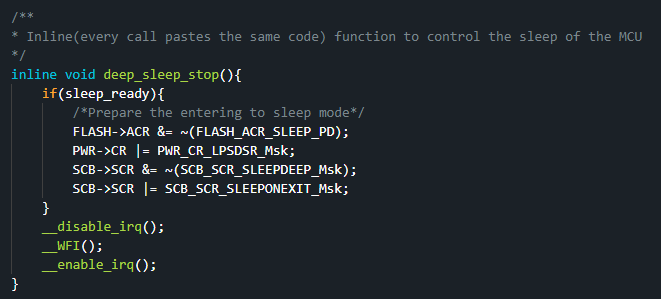
\includegraphics[width=0.8\textwidth]{images/5/Low Power.png}
    \caption{Low power mode function of the system}
    \label{fig:lowPower}
\end{figure}
\begin{itemize}
    \item First, the Flash is configured to power on in sleep mode.
    \item Second, the voltage regulator is put in a low-power state during sleep mode.
    \item Third, the low-power mode is configured for the sleep mode.
    \item Finally, the system will re-enter sleep mode when coming from an \acrshort{isr}.
\end{itemize}

\subsection{Interruption management}

As explained in the next chapter, the color sensor wasn't able to generate interruptions.

To compensate for this, an orientation detection was implemented with the accelerometer. To make this, the accelerometer initialization was changed:
\begin{itemize}
    \item The interruptions on orientations were activated and mapped to PIN2 of the accelerometer sensor.
    \item As we are working with orientation changes, if we don't work around fast changing orientations, we will have problems. To solve this, the internal debounce counter of the accelerometer was put to \texttt{100ms}.
    \item Finally, we clean a first interruption that happens at start of the accelerometer. This is done automatically by reading one specific register.
\end{itemize}

Finally, \autoref{fig:advancedSerial} presents the end result of data sent to the computer. Also, when some orientation change is detected, it is also sent to the computer.
\begin{figure}[H]
    \centering
    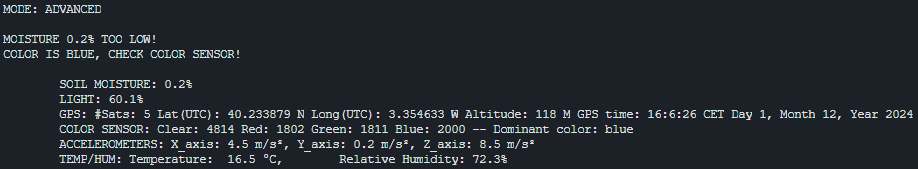
\includegraphics[width=0.99\textwidth]{images/5/AdvancedSerial.png}
    \caption{Advanced information sent to the computer}
    \label{fig:advancedSerial}
\end{figure}
